\documentclass[12pt,a4paper]{article}
\usepackage[a4paper,vmargin={1in,1in},hmargin={1.25in,1in}]{geometry}	% Setup of page size,margins
\usepackage{graphics}
\usepackage[font=small,labelfont=bf]{caption}
\usepackage{fancybox}		% For formatting of cover page5
\usepackage{amsmath}    	% For  mathematical formulae
\usepackage{amsfonts}
\usepackage{amssymb}
\usepackage{setspace}		% For adjusting line spacing 
\usepackage{pdfpages}
\usepackage[square, comma, sort&compress,numbers]{natbib} % For customizing citations
\usepackage[pdftex]{hyperref}	% For having working URLs for references 
\usepackage{chngcntr,tocloft}
\counterwithin*{figure}{subsubsection}
\renewcommand{\thefigure}{%
      \thesubsubsection.\arabic{figure} %
      }
\begin{document}
\pagenumbering{roman}
\pagestyle{empty}
%---------------------------------------------------------------------------------------------------------

\newpage
\pagestyle{empty}
\pagenumbering{gobble}
%\thisfancypage{cmds1}{cmds2}
\thisfancyput(-0.0 in, -10.0 in) {\setlength{\unitlength}{1 in}\framebox(6.7,10.2)}
 
 \begin{center}
      
      \textbf{A PROJECT REPORT}\\
      \vspace{0.2 in}
      \textbf{ON}
      \vspace{0.2 in}
       
			\end{center}
\vspace{0.1 in}
	\begin{center}
		\textbf{ROVER THERAPIST}\\
	\end{center}
     \vspace{0.2 in}
		\begin{center}
	    SUBMITTED TO THE UNIVERSITY OF PUNE \\
	    IN PARTIAL FULFILLMENT OF THE REQUIREMENTS\\
	    FOR THE AWARD OF THE DEGREE \\
	    \\
	    OF\\
	    \\
	    \textbf{B.E.(INFORMATION TECHNOLOGY)}
	\end{center}
	
	\vspace{0.2 in}
	
	\begin{center}
	   \textbf{SUBMITTED BY}
	\end{center}
	\vspace{0.1 in}
	\begin{center}
	\textbf{SHUBHAM CHANDAK  47008}\\
	\textbf{RIDHIMA JOSHI  47020}\\	
	\textbf{MADHUR LAHOTI  47028}\\
	\end{center}
	
	 \vspace{0.2 in}
	\begin{center}
	    UNDER THE GUIDANCE OF \\
	    \\
	    \\
	    \textbf{PROF. C.A.GHUGE}\\
	    \\
	    \\
	    \textbf{DEPARTMENT OF INFORMATION TECHNOLOGY}\\
	    \\
	    \textbf{P.E.S's}\\
	    \textbf{MODERN COLLEGE OF ENGINEERING,}\\
	    \textbf{SHIVAJINAGAR, PUNE-411005}\\
	    \\
	    \textbf{UNIVERSITY OF PUNE}\\
	    \\
	    \textbf{*2014-2015*}\\
	     \end{center}

%---------------------------------------------------------------------------------------------------------
\newpage
\pagestyle{empty}
 %\thispagestyle{empty}
	\pagenumbering{gobble}
	\thisfancyput(-0.0 in, -10.0 in) {\setlength{\unitlength}{1 in}\framebox(6.7,10.2)}
\begin{center}
      
      \textbf{A PROJECT REPORT}\\
      \vspace{0.2 in}
      \textbf{ON}
      \vspace{0.2 in}
       
			\end{center}
\vspace{0.1 in}
	\begin{center}
		\textbf{ROVER THERAPIST}\\
	\end{center}
     
	\vspace{0.2 in}
	
	\begin{center}
	   \textbf{SUBMITTED BY}
	\end{center}
	\vspace{0.1 in}
	\begin{center}
	\textbf{SHUBHAM CHANDAK  47008}\\
	\textbf{RIDHIMA JOSHI  47020}\\	
	\textbf{MADHUR LAHOTI  47028}\\
	\\
	\textbf{B.E.(INFORMATION TECHNOLOGY)}\\
	\\
	\begin{center}
	UNDER THE GUIDANCE OF\\
	\\
	\end{center}
	\textbf{PROF. C.A GHUGE}\\
	\\
	\end{center}
	
	\begin{center}

\includegraphics[width=2.5cm]{modernlogo}
\end{center}
	\begin{center}
	
	
\textbf {DEPARTMENT OF INFROMATION TECHNOLOGY }\\
\\
\textbf {P.E.S's}\\
\textbf{ Modern College Of Engineering,} \\
\textbf{Shivajinagar,Pune-5}\\
\\
\textbf{UNIVERSITY OF PUNE}\\
\\
\textbf{*2014-2015*}\\
\end{center}

%---------------------------------------------------------------------------------------------------------
\newpage
\pagestyle{empty}
 %\thispagestyle{empty}
	\pagenumbering{gobble}
	\thisfancyput(-0.0 in, -10.0 in) {\setlength{\unitlength}{1 in}\framebox(6.7,10.2)}

\vspace{0.2in}
\begin{center}
\textbf{\large{Progressive Education Society's}}\\
\textbf{\large{Modern College of Engineering, Shivajinagar,}}\\
\textbf{\large{Pune-411005.}}\\
\\
\\
\vspace{0.2in}
\end{center}

	\begin{center}

\includegraphics[width=2.5cm]{modernlogo}
\end{center}

\begin{center}
\textbf{\large{CERTIFICATE}}\\
\end{center}

		\noindent
  				\setlength{\baselineskip}{1.5\baselineskip}
	\begin{center}
\begin{flushleft}
This is to certify that the following students of Final Year Information Technology have successfully completed the project entitled \textbf{\small"ROVER THERAPIST"}in the academic year 2014-2015.\\
The Group Members name are: Shubham Chandak\\
		\hspace{5.76 cm}					Ridhima Joshi\\
		\hspace{5.76 cm}					Madhur Lahoti\\
\\
\end{flushleft} 

\begin{flushleft}
This is partial fulfillment of Bachelor of Information Technology under the University of Pune,Pune.

\\
Date:
\\
\end{flushleft}
	\end{center} 
		\vspace{0.6 in}
(Prof.Mrs.S.D.Deshpande)\hspace{2.8 in} (Prof. C.A. Ghuge)\\
HOD of Department\hspace{1 in} External Examiner\hspace{1 in}  (Internal Guide)\\
(Information Technology)\\\\\
\singlespace

%---------------------------------------------------------------------------------------------------------

\newpage
\pagenumbering{roman}
\addcontentsline{toc}{section}{ACKNOWLEDGMENT}
\pagestyle{plain}           %For displaying roman page nos
\begin{center}
\bf ACKNOWLEDGEMENT
\end{center}
\hspace{0.7cm}We take this opportunity to express our sincere thanks to our project guide Prof. C. A. Ghuge and Head of the Department Prof. Mrs. S. D. Deshpande for their valuable time and guidance and for providing all the necessary facilities, which were indispensable in the completion of this project report. 

We are also thankful to all the staff members of the Department of Information Technology of Modern College of Engineering, Pune for their valuable time, support, comments, suggestions and persuasion.

We would also like to thank the institute for providing the required facilities, Internet access and important books.
  
We would also like to thank our colleagues and friends for their support and timely suggestions.

\begin{flushright}
\hspace{3.5in} 
Shubham Chandak\\
Ridhima joshi\\	
Madhur Lahoti\\
\end{flushright}

%---------------------------------------------------------------------------------------------------------

\newpage
\addcontentsline{toc}{section}{ABSTRACT}
\pagestyle{plain}           %For displaying roman page nos
\begin{center}
\bf ABSTARCT
\end{center}
\hspace{0.7cm}Customer Relationship Management (CRM) is currently one of the most used notions in articles and studies dealing with computer applications. Nowadays it is very difficult for a company to convince a customer (a potential client) with only product or price arguments because of the strong competition in almost all market areas. Aim of our project deals with finding tourist attractions, optimal path finding for tourist attraction, suggestions for way of transportation, seasonal classification and calculation of the fare using distance formula calculation. This project also helps the tourist to lodge a complaint against the Tourist Guide’s, Rented vehicle drivers for diverting the tourist and charging him unfair tariff & finding out emergency numbers for the particular city. Based on the complaint lodged by the passenger the reports are generated and submitted to the higher authorities. Whenever user reaches near to the tourist place images of that place pops up on his phone. Tourist will get the places list as per his location and places are fetched from database as well as Google. Seasonal classification of places is also provided i.e. places to be visited in summer season, winter season and rainy season, this feature will suggest user to visit that particular place which must be visited during that season.

%---------------------------------------------------------------------------------------------------------
\\

\newpage
{\setlength{\baselineskip}{1.5\baselineskip}
\tableofcontents
}

%---------------------------------------------------------------------------------------------------------
\newpage
{\setlength{\baselineskip}{1.5\baselineskip}
\listoftables
\addcontentsline{toc}{section}{LIST OF TABLES}
}

%---------------------------------------------------------------------------------------------------------

\newpage
{\setlength{\baselineskip}{1.5\baselineskip}
\listoffigures
\addcontentsline{toc}{section}{LIST OF FIGURES}
}

\newpage
{\setlength{\baselineskip}{1.5\baselineskip}
\listoffigures
\addcontentsline{toc}{section}{LIST OF FIGURES}
}

%---------------------------------------------------------------------------------------------------------
\newpage
\pagenumbering{arabic}
\pagestyle{plain} 
\begin{center}
\section{INTRODUCTION}
\end{center}
\\
\\
\subsection{INTRODUCTION}
\hspace{0.7 cm}Our application is based on mobile CRM concept which will help the user.
\\
\subsubsection{PURPOSE}
\\
\hspace{0.7 cm}Aim of this project deal with finding tourist attractions, optimal path finding for tourist attraction, suggestions for way of transportation, and if the tourist is opting for Rented Vehicle then calculation of the fare using optimal path distance calculation provided by Google Maps API. This project also helps the tourist to lodge a complaint against the Tourist Guide’s, Vehicle Drivers for Diverting the tourist and charging him unfair tariff & finding out emergency numbers for the particular city.
\\
\subsubsection{OVERVIEW}
\\
Using this application user can detect source of user and from there he can get nearest tourist places in his area. User also can find the multiple routes, available transport facility and fair calculation. The data found on this app is more than Google. In current scenario some application shows the data which only available  on Google, in these app there is no local places on Google, so we are trying to give the data of local places also which are not much popular on Internet with detail information.  
\\
\subsubsection{BUSINESS CONTEXT}
\\
\begin{enumerate}
\item Future Mobile Customer Relationship Management in the automotive industry and the tourism. The key profiles of future mobile communication are Interactive Broadband Protocols, Location Based Services and Individualized/Personalized Services mainly based on Multimedia information. These profiles are embedded in a three layer communicate model.
\\
\item The grade of customer’s satisfaction is most relevant factor for the breakdown or the success of a company. 
\\
\item Aim of this project deal with finding tourist attractions, optimal path finding for tourist attraction, suggestions for way of transportation, and if the tourist is opting for Rented Vehicle then calculation of the fare using optimal path distance calculation provided by Google Maps API.
\\
\item This project also helps the tourist to lodge a complaint against the Tourist Guide’s, Rented Vehicle Drivers for diverting the tourist and charging him unfair tariff & finding out emergency numbers for the particular city.
\end{enumerate}
\\
\subsection{PROBLEM STATEMENT}
\\
\hspace{0.7 cm}To develop an android application for tourists who are exploring the city. To help the tourists search for places and provide security like lodging complaint against the drivers. To detect the distance of the destination from the source using distance algorithm.
\\
\subsection{PROJECT SCOPE}
\\
\hspace{0.7 cm}This project will aim at developing an android application which will help the user to locate the nearby places. The application will use the Goople API to display the places and distance algorithm to calculate the distance from source to destination.
\\
\hspace{0.7 cm}When the user opens the application source of the user will be detected. The user can select the categories which he wants to visit.This will show the places according to the categories selected. The places will also be shown as per the current weather. The algorithm will calculate the fare as per the distance.
\\
\hspace{0.7 cm} According to weather places will be suggested to the user also.
\subsection{PROJECT OBJECTIVES}
\\
\hspace{0.7 cm}Our project aims at delivering an application to the customer where he can use it whenever he visits the city. Project objectives are:
\begin{enumerate}
\item Detecting the source of the user.
\\
\item Listing of tourist places.
\\
\item Calculating fare according to the distance.
\\
\item Lodge a compliant.
\\
\item Show places according to the weather.
\\
\item Places are fetched from database as well as Google.
\\
\item Places can be sorted as per the categories.
\end{enumerate}
\\
\subsection{ASSUMPTIONS AND DEPENDENCIES}
\\
\hspace{0.7 cm} For the application to run following constraints should be present:-
\subsubsection{Assumptions}
\\
\begin{enumerate}
\item The device on which the application is running should be a android device.
\item User must have basic knowledge to operate android phone.
\end{enumerate}
\\
\\
\subsubsection{Dependencies}
\\
\begin{enumerate}
\item The device should have the facility of GPS.
\item The device should be connected to the internet.
\end{enumerate}
\\
\subsection{LITERATURE SURVEY}
\\ 
\hspace{0.7 cm}Literature survey is the most important step in software development process. Before developing the tool it is necessary to determine the time factor, economy n company strength. Once these things are satisfied, ten next steps are to determine which operating system and language can be used for developing the tool. Once the programmers start building the tool the programmers need lot of external support. This support can be obtained from senior programmers, from book or from websites. Before building the system the above consideration are taken into account for developing the proposed system.
\\
\subsubsection{Customer Relationship Management Using Android Phone in Tourism}

\textbf{Authors:	Nitin Khondre, Ravi Saini, Ronak Jain,Sarang Suryawanshi, Bushra Quazi}
\\
\textbf{Year:		March 2014}
\\
\textbf{Journal: 	International Journal of Emerging Technology and Advanced Engineering}
\\
\textbf{Website: www.ijetae.com (ISSN 2250-2459, ISO 9001:2008 Certified Journal, Volume 4, Issue 3, March 2014)}
}
\\
\hspace{0.7 cm}Customers are the vital key for each business and company to help them to grow. So, implementing CRM important tools that will help managers and companies to increase the satisfaction and loyalty of customers more than before. Nowadays it is very difficult for a company to convince a customer with only product or price arguments because of the strong competition in almost all market areas. Mobile technology offers a high potential to significantly transform the ways how a company can interact  with their customers and even with own employees. Therefore, this paper deals with the possibilities and aspects to support CRM via future mobile services.^{[1]}


\subsubsection{inGuide-Interactive Guide}

\textbf{Authors: 	Filipe Andre Gomes Batista, Nuno Rodrigues, and Alexandrino Goncalves}
\\
\textbf{Year: 		2009}
\\
\textbf{Journal:  3rd IEEE International Conference on Digital Ecosystems and Technologies Future Mobile CRM in Automotive and Tourist Area}
}
\\
\hspace{0.7 cm}This paper describes the inGuide modular application which provides a package management system avoiding the need for a different version of the application for each city. It also describes the geolocation technology in order to provide contextual information in a simple and interactive way. This paper describes two modes those are online mode and offline mode. We preferred online mode of GPS tracking as it gives more accurate location.^{[2]}  
\\

\subsubsection{On-line GPS Track Simplification Algorithm for Mobile Platforms}

\textbf{Author:	R. Ivanov}
\\
	\textbf{Year:		2010}
\\
	\textbf{Journal:	Information Technology and Control}
}
\\
\hspace{0.7 cm}This paper describes an algorithm for on-line simplification of the number of points, describing a GPS track. It is offered on the base of analysis of the location of three last points and calculation by basic trigonometric ratios and distance formula.^{[3]}
\\

\subsubsection{Overview on Android- The New Mobile Operating System}
\\
\textbf{Author:	Monika Bazard, Sonia Bhardwaj}
\\
\textbf{Year:		April, 2011}
\\
\textbf{Journal:	SGI Reflections- International Journal of Science, Technology and Management. ISSN No. 0976-2140. Volume 2, Issue 1, April, 2011}
\\
\hspace{0.7 cm}This paper describes the Android’s history, architecture, libraries and its advantages and disadvantages in the smart phones.^{[4]}
\\

%---------------------------------------------------------------------------------------------------------
\newpage
\begin{center}
\pagestyle{plain} 
\section{PROJECT PLAN}
\end{center}
\hspace{0.7cm}\\
\pagestyle{plain} 
\subsection{TASK SHEET SCHEDULE}
We performed the following tasks:
\begin{center}
\vspace{0.1cm}

\newpage
\begin{table}
\begin{tabular}{| p{4 cm}| p{2 cm}| p{2 cm}| p{2 cm}|}
\hline
\textbf{TASK NAME} & \textbf{TASK DURATION} & \textbf{START DATE} & \textbf{END DATE} &
\hline
Search for BE project topics and related papers & & & &
\hline
Short listing of topics & & & &
\hline
Presentation of topic to the project coordinator and final selection of topic & & & &
\hline
Submission of base paper and synopsis & 2 days & 30/08/2014	& 1/09/2014 &
\hline
Discussion on SRS and implementation of SRS & 2 days & 9/09/2014 & 11/09/2014 &
\hline
Corrections in SRS and implementation of UML diagram & 2 days & 18/09/2014 & 20/09/2014 &
\hline
Discussion on literature survey and SRS format & 2 days	&  & 25/09/2014 &
\hline
Preparation of Partial report in latex & 8 days	& & 9/10/2014 &
\hline
Partial report submission and signing & 1 day & 17/10/2014 & 17/10/2014 &
\hline
Semester VII project viva & 1 day & /10/2014 & /10/2014 &
\hline
Discussion on what to do in semester VIII & 1 day & 22/12/2014 & 22/12/2014 &
\hline
Changes in Admin Module and rough ER & 2 days & 09/01/2015 & 11/01/2015 &
\hline
Part of Android application discussed with project guide & 5 days & 14/01/2015 & 19/01/2015 &
\hline
Working on database & 15 days & 08/01/2015 & 23/01/2015 &
\hline
Completion of Admin module & 15 days & 08/01/2015 & 23/01/2015 &
\hline
Review I of project & 1 day & 28/01/2015 & 28/01/2015 &
\hline
Discussion on class diagram & 1 day & 23/02/2015 & 23/02/2015 &
\hline
Preparation of Final report in latex & 11 days & 1/03/2015 & 11/03/2015 &
\hline
Shown Android module to the project guide & 1 day & 16/03/2015 & 16/03/2015 &
\hline
Showed the changes in the project to the project guide & 8 days	& 20/03/2015 & 27/03/2015 &
\hline
Review II of project & 1 day & 28/03/2015 & 28/03/2015 &
\hline
Discussion on some points of report and changes in the report & 2 days & 28/03/2015 & 30/03/2015 &
\hline
Final Report submission signing & 1 day & 15/04/2015 & 15/04/2015 &
\hline
\end{tabular}
\caption{Task Sheet Schedule}
\end{table}
\\
\end{center}
%-------------------------------------------------------------------------------------------------
\newpage
\pagestyle{plain} 
\begin{center}
%srs
\section{REQUIREMENT ANALYSIS}  
\end{center}
\\
\subsection{HARDWARE REQUIREMENTS}
\\
\hspace{0.7 cm} The system requires following hardware requirements:
\\
\begin{enumerate}
\item System:	Intel P4, 2.4 GHZ, 40 GB HDD for installation. 
\\
\item Memory:	512 MB memory, 256 MB ram 
\\
\item Project’s server side system is windows based supporting versions windows XP onwards.  

\end{enumerate}
\\
\\
\subsection{SOFTWARE REQUIREMENTS}
\\
\begin{enumerate}
\item 	Eclipse 3.7 Indigo
\item Android SDK
\item Android 2.3
\item Android GPS API
\item Apache Tomcat Server
\item MySQL
\end{enumerate}
\\
%---------------------------------------------------------------------------------------------------------
\newpage
\pagestyle{plain} 
\begin{center}
\section{PROJECT DESIGN}
\end{center}
\hspace{0.7cm}
\\
\subsection{E-R DIAGRAM}
\begin{figure}[!htb]
\centering
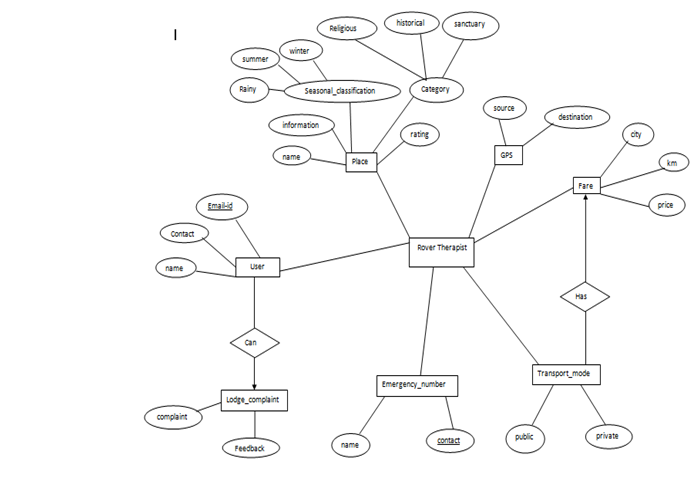
\includegraphics[width=12 cm]{er}
\caption{ER Diagram}
\end{figure}
\\
\newpage
\subsection{DATA FLOW DIAGRAMS}
\\
\subsubsection{DFD LEVEL0}
\begin{figure}[!htb]
\centering
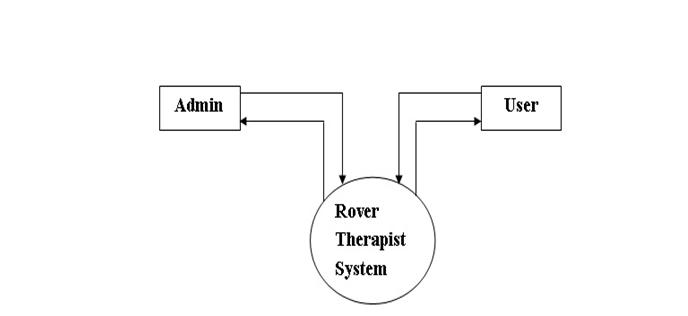
\includegraphics[width=15 cm]{level}
\caption{DFD Level 0}
\end{figure}
\\
\newpage
\subsubsection{DFD LEVEL1}
\begin{figure}[!htb]
\centering
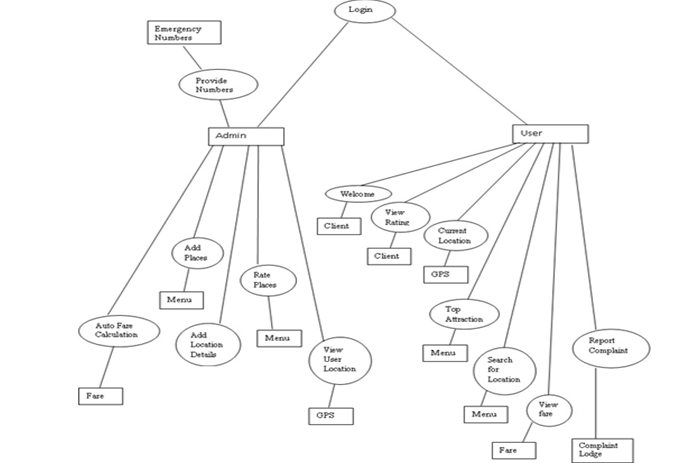
\includegraphics[width=15 cm]{levell}
\caption{DFD Level 1}
\end{figure}
\\
\newpage
\subsection{UML DIAGRAMS}
\\
\subsubsection{USE CASE DIAGRAM}
\begin{figure}[!htb]
\centering
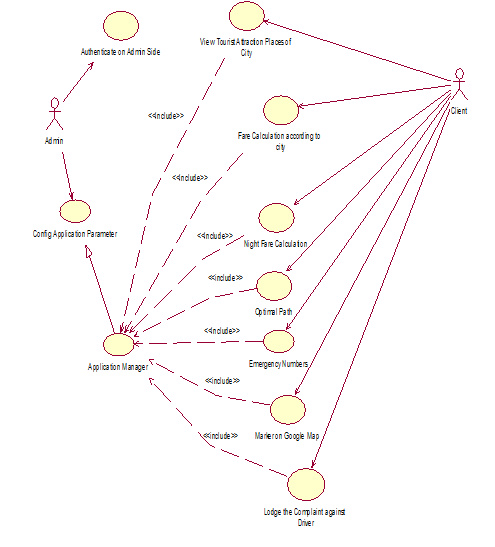
\includegraphics[width=15 cm]{UseCase}
\caption{Use Case Diagram}
\end{figure}
\\
\newpage
\subsubsection{CLASS DIAGRAM}
\begin{figure}[!htb]
\centering
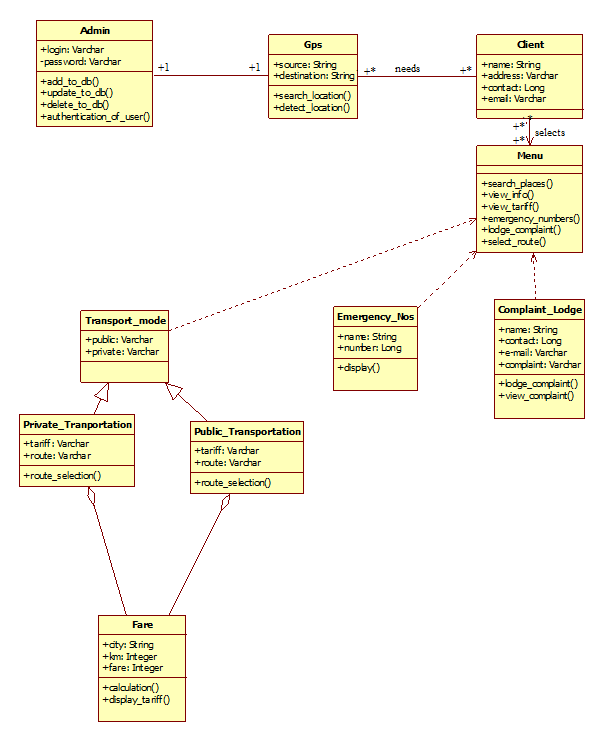
\includegraphics[width=15 cm]{class}
\caption{Class Diagram}
\end{figure}
\\
\newpage
\subsubsection{ACTIVITY DIAGRAM}
\begin{figure}[!htb]
\centering
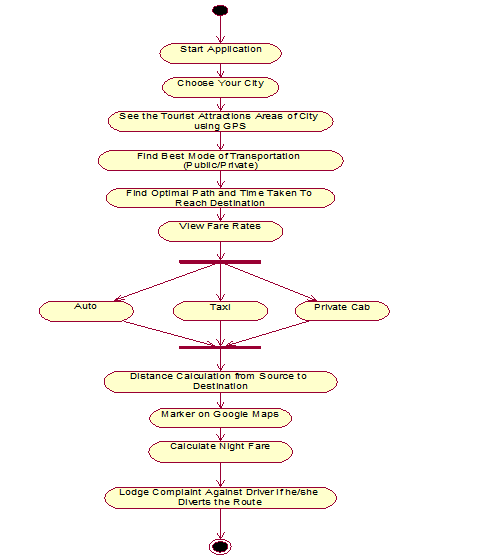
\includegraphics[width=15 cm]{activity}
\caption{Activity Diagram}
\end{figure}
\\
\newpage
\subsubsection{PACKAGE DIAGRAM}
\begin{figure}[!htb]
\centering
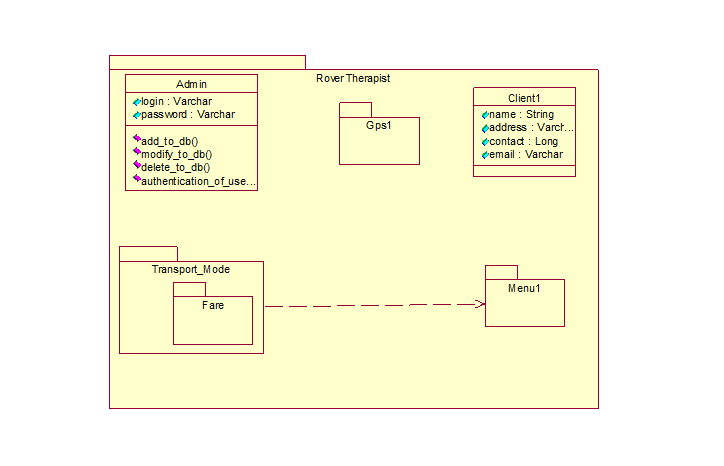
\includegraphics[width=15 cm]{package}
\caption{Package Diagram}
\end{figure}
\\
\newpage
\subsubsection{SEQUENCE DIAGRAM}
\begin{figure}[!htb]
\centering
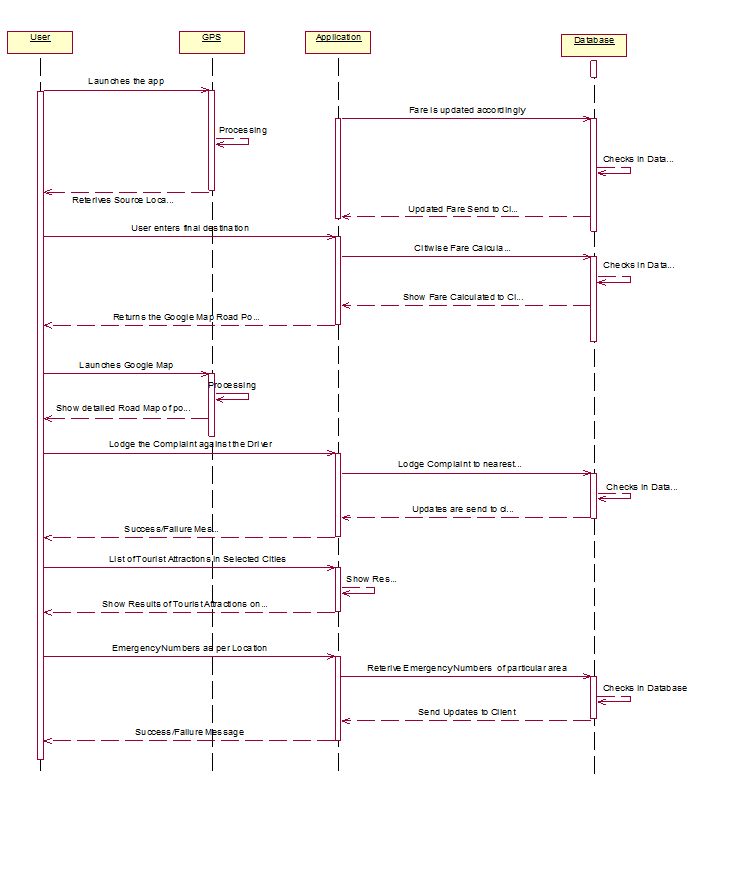
\includegraphics[width=15 cm]{Seq}
\caption{Sequence Diagram}
\end{figure}
\\
\newpage
\subsubsection{COMMUNICATION DIAGRAM}
\begin{figure}[!htb]
\centering
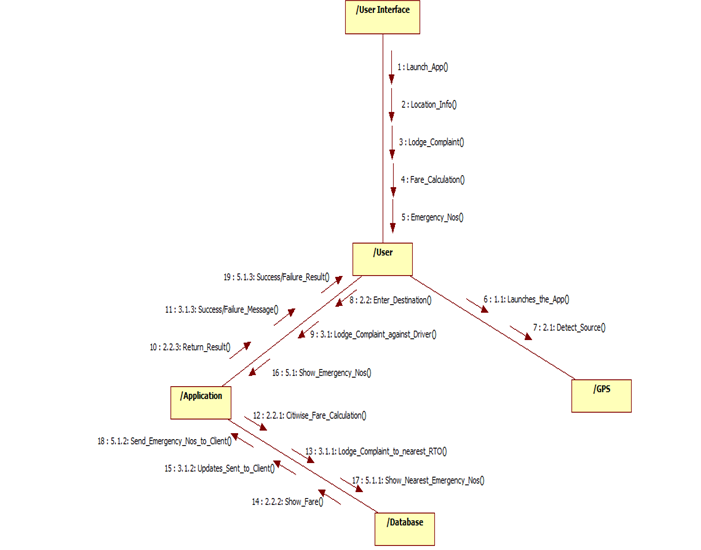
\includegraphics[width=15 cm]{communication}
\caption{Communication Diagram}
\end{figure}
\\
\newpage
\subsubsection{COMPOSITE STRUCTURE DIAGRAM}
\begin{figure}[!htb]
\centering
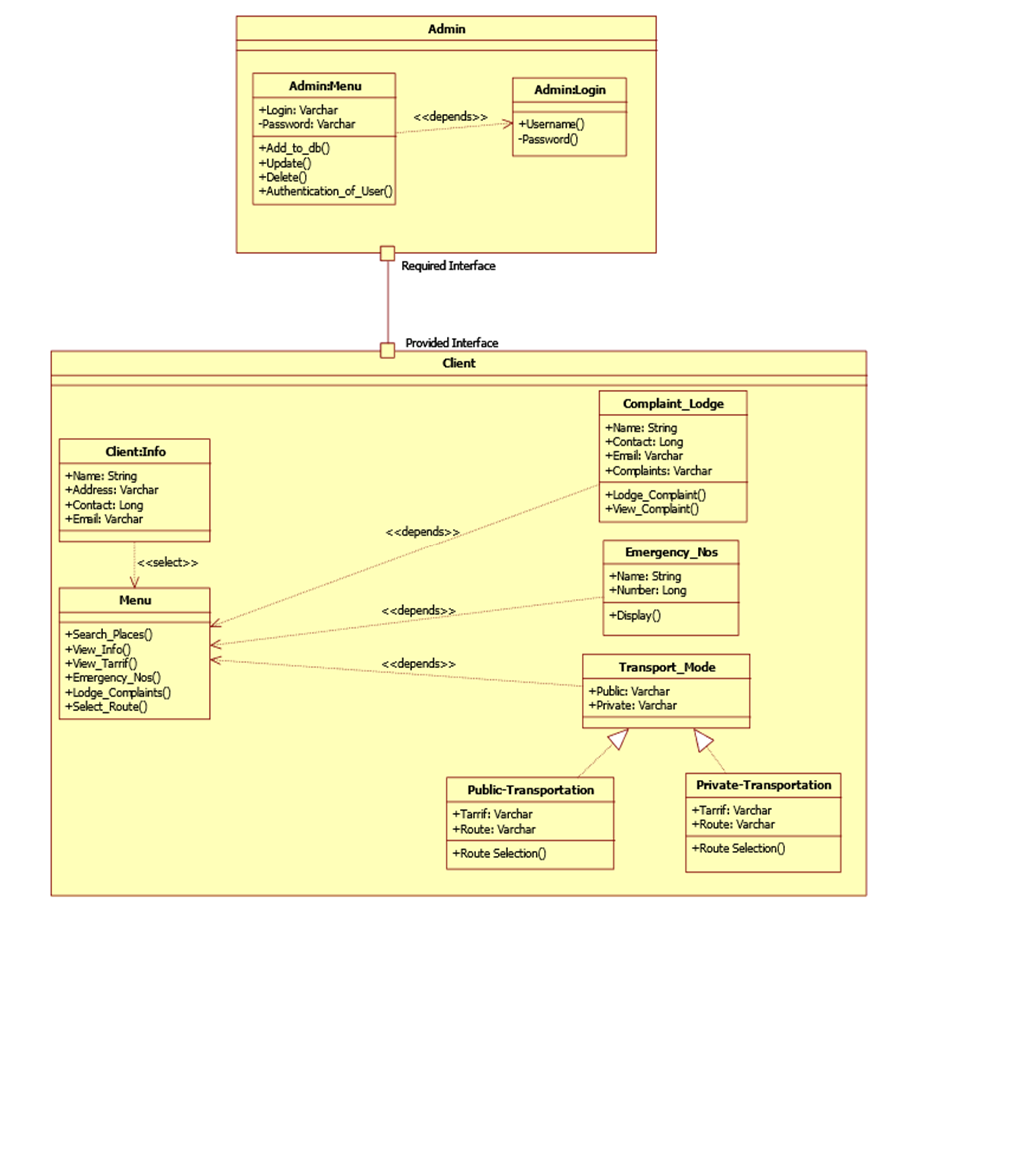
\includegraphics[width=15 cm]{composite}
\caption{Composite Structure Diagram}
\end{figure}
\\
\newpage
\subsubsection{STATE MACHINE DIAGRAM}
\begin{figure}[!htb]
\centering
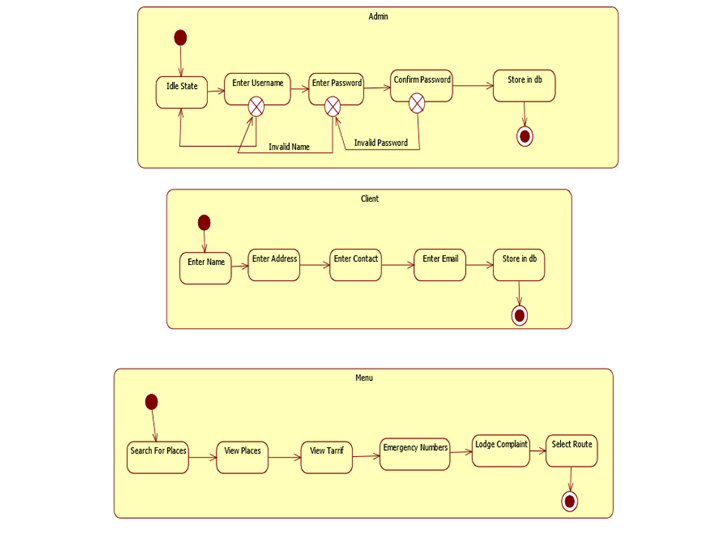
\includegraphics[width=15 cm]{state}
\caption{State Machine Diagram}
\end{figure}
\\
\newpage
\subsubsection{COMPONENT DIAGRAM}
\begin{figure}[!htb]
\centering
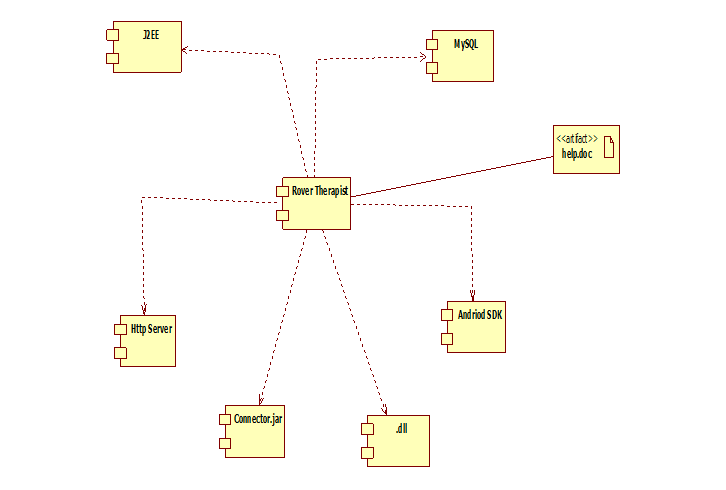
\includegraphics[width=15 cm]{component}
\caption{Component Diagram}
\end{figure}
\\
\newpage
\subsubsection{DEPLOYMENT DIAGRAM}
\begin{figure}[!htb]
\centering
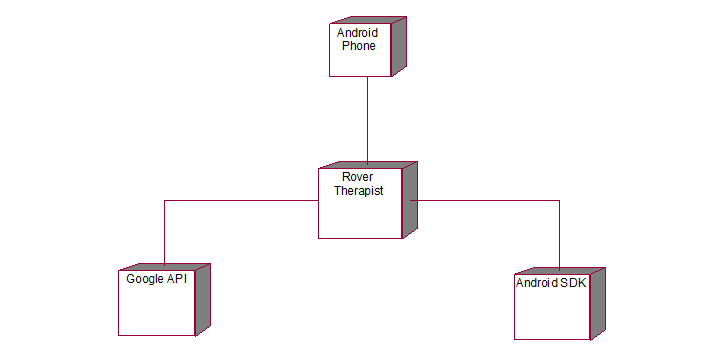
\includegraphics[width=15 cm]{deployment}
\caption{Deployment Diagram}
\end{figure}
\\

%---------------------------------------------------------------------------------------------------------
\newpage
\pagestyle{plain}
\begin{center}
\section{IMPLEMENTATION DETAILS}
\end{center} 
\\
\subsection{PROJECT ARCHITECTURE}
\hspace{0.7 cm} Our application has a three-tier architecture. It has three layers:

\begin{enumerate}

\item Presentation Layer
It provides user interface. It handles the interaction with the user.

\item Logic Layer
Contains the business logic.

\item Data Layer
It is the physical storage layer for data persistence. It manages access to the database.
\end{enumerate}	
\\
\subsection{ALGORITHM}
\textbf{DISTANCE BASED ALGORITHM}
\\
\hspace{0.7 cm} The distance based algorithm used is the Hoversine algorithm. Hoversine algorithm uses the latitude and longitude for calculation of distance from the GPS. It calculates the shortest distance between the two points.
\\
\textbf{Haversine Formula:}
\\
	a=〖sin〗^2(∆∅/2)+cos∅_1.cos∅_2.〖sin〗^2(∆⋋/2)
	\\
           c=2.atan2(√(a,) √((1-a)) )
           \\
           d=R.c
\\
where ∅ is latitude,
\\
            ⋋ is longitude,
            \\
             R is earth’s radius (mean radius =6,371 km)
\\
\textbf{Implementation of Algorithm:}
\\
public static double calcDistance(double lat_a, double lng_a, double lat_b,double lng_b) {
\\
			float pk = (float) (180 / Math.PI);
\\
			double a1 = lat_a / pk;
			\\
			double a2 = lng_a / pk;
			\\
			double b1 = lat_b / pk;
			\\
			double b2 = lng_b / pk;
\\
double t1 = (double) (Math.cos(a1) * Math.cos(a2) *          Math.cos(b1) * Math.cos(b2));
\\
double t2 = (double) (Math.cos(a1) * Math.sin(a2) * Math.cos(b1) * Math.sin(b2));
\\
			double t3 = (double) (Math.sin(a1) * Math.sin(b1));
\\
			double tt = Math.acos(t1 + t2 + t3);
\\
			return 6366000 * tt;
			\\
	}
\\
\newpage
\subsection{TECHNOLOGIES, TOOLS AND LIBRARIES USED}
\\
\subsubsection{TECHNOLOGIES}
\\
\begin{enumerate}
\item \textbf{JAVA}
\\
\hspace{0.7 cm} Java is a general-purpose computer language that is concurrent, class-based, object-oriented. It contains features like classes, objects, encapsulation, abstraction, inheritance and polymorphism. Java is designed by James Gosling and Sun Microsystems. Java is simple, robust, secure, system independent language, portability, interpreted, multithreaded. Sun Microsystems Inc. has divided Java into three parts - Java SE, Java EE and Java ME.^{[5]}
\\
\begin{itemize}
\\
\item \textbf{Java SE:}
\\
\hspace{0.7 cm} It is the Java Standard Edition that contains basic core java classes. This edition is used to develop standard applets and applications.
\\
\item \textbf{Java EE:}
\\
\hspace{0.7 cm} It is the Java Enterprise Edition and it contains classes that are beyond Java SE. To use many of the classes in Java EE, Java SE is used. It mainly concentrates on providing business solutions on a network.
\\
\item \textbf{Java ME:}
\\
\hspace{0.7 cm} It stands for Java Micro Edition. It is for developers who develop code for portable devices, such as a PDA or a cellular phone.
\\
\end{itemize}
\\
\item \textbf{HTML}
\\
\hspace{0.7 cm} HTML is a markup language commonly used to create Web pages. A markup language provides a way to describe the structure of text and graphics on a Web page. It is developed and maintained by World Wide Web consortium (W3C). The term hyper signifies the navigation from one location to another in a non-linear fashion. HTML defines the content, i.e. the structure and the layout of a Web page with the help of elements and attributes. An element includes the start and the end tags, with some content within them, and attributes provide additional information about the elements.^{[6]}
\\
\item \textbf{CSS}
\\
\hspace{0.7 cm} CSS is a style sheet language that is used to describe the apperance and formatting of a Web document, which is written in a markup language. It enables one to keep separate the instructions related to the presentation of Web content fron the Web content itself.
\\
\hspace{0.7 cm} A CSS style sheet consists of a list of rules, which in turn consists of one or more selectors and a declaration block. Selectors are used to declare the mark elements to which a style applies to, while a declaration block consists of a list of declarations in braces.^{[7]}
\\
\item \textbf{Servlet}
\\
\hspace{0.7 cm} A servlet is a simple Java class, which is dynamically loaded on a Web server and thereby enhances the functionality of the Web server. Servlets are secure and portable as they run on JVM embedded with the Web server and cannot operate outside the domain of the Web server. That is servlets are objects that generate dynamic content after processing requests that originate from a Web browser. They are Java components that are used to create dynamic Web applications. Servlets can run on any Java-enabled platform and are usually designed to process HTTP requests, such as GET and POST.^{[8]}
\\
\item \textbf{Javascript}
\\
\hspace{0.7 cm} JavaScript is an object-oriented scripting language that is used to design interactive websites. It is developed by Netscape and works in all major browsers, such as Internet Explorer, Firefox, Chrome, Opera, and Safari. It is used with HTML code to add dynamic content to their websites. It is an interpreted language.^{[9]}
\\
\item	\textbf{Android}
\\
\hspace{0.7 cm} Android is an operating system based on Linux with Java programming interface. It provides tools such as a compiler, debugger and a device emulator as well as JVM. It is created by the Open Handset Alliance which is lead by Google.^{[10]}
\\
\hspace{0.7 cm} Android uses a special virtual machine, e.g. the Dalvik Virtual Machine. dalvik uses special bytecode. Therefore one cannot run standard of Java bytecode on Android. It provides a tool "dx" which allows conerting Java Class files into "dex" files. Android applications are packed into an .apk(Android Package) file.
\\
\hspace{0.7 cm} Every Android application runs in its own process and under its own user id which is generated automatically by the Android system during deployment. Therefore the application is isolated from other running applications and a misbehaving applications cannot easily harm other Android application.
\\
\textbf{ANDROID DEVELOPMENT TOOLS}
\\
\hspace{0.7 cm}	Google provides the ADT to develope Android applications with Eclipse. ADT is a set of components (plug-ins) which extend the Eclipse IDE with Android development capabilities. 
\\
\hspace{0.7 cm}	ADT contains all required functionalities to create, compile, debug and deploy Android applications from the Eclipde IDE. It also allows creating and starting AVDs.
\\
\\
\textbf{ANDROID SDK}
\\
\hspace{0.7 cm}The Android Software Development Kit(SDK) contains the necessary tools to create, compile and package Android application. Most of these tools are command line based.
\\
\hspace{0.7 cm}It also provides an Android device emulator, so that Android application can be tested without a real Android phone. AVD (Android Virtual device) via the Android SDK can be created, which run in the emulator.
\\
\hspace{0.7 cm} It contains the Android debug bridge (adb) tool which allows to connect to an virtual or real Android device.
\\
\item \textbf{JSON(JavaScript Object Notation)}
\\
\hspace{0.7 cm}JSON is a lightweight data-interchange format. It is easy for humans to read and write. It is easy for machines to parse and generate. It is a text format that is completely language independent but uses conventions that are familiar to programmers of the C-family of languages, including C, C++, C#, Java, JavaScript, Perl, Python, and many others. These properties make JSON an ideal data-interchange language.^{[11]}
\\
\hspace{0.7 cm}JSON is built on two structures:
\\
\begin{itemize}
\item	A collection of name/value pairs. In various languages, this is realized as an object, record, struct, dictionary, hash table, keyed list, or associative array.

\item	An ordered list of values. In most languages, this is realized as an array, vector, list, or sequence.
\end{itemize}

\textbf{Example of JSON describing a person:}
\\
\hspace{0.7 cm}	{\\
\hspace{0.7 cm}		 “firstName” : “John” ,\\
\\
\hspace{0.7 cm}	     	 “lastName” : “Smith” ,\\
\\
\hspace{0.7 cm}	      	 “isAlive” : true ,\\
\\
\hspace{0.7 cm}	      	 “age” : 25 ,\\
\\
\hspace{0.7 cm}		“height_cm” : 167.6 ,\\
\\
\hspace{0.7 cm}		“address” : {\\
\\
\hspace{0.7 cm}			“streetAddress” : “21 2nd Street” ,\\
\\
\hspace{0.7 cm}			“city” :  “New York” ,\\
\\
\hspace{0.7 cm}			“state” : “NY” ,\\
\\
\hspace{0.7 cm}			“postalCode” : “10021-3100”\\
\\
\hspace{0.7 cm}			      } ,\\
\\
\hspace{0.7 cm}		“phoneNumbers” : [\\
\\
\hspace{0.7 cm}		{\\
\\
\hspace{0.7 cm}			“type” : ”home” ,\\
\\
\hspace{0.7 cm}			“number” :”212 555-4567”\\
\\
\hspace{0.7 cm}		}\\
\\
\hspace{0.7 cm}		],\\
\\
\hspace{0.7 cm}		“children” : [ ] ,\\
\\
\hspace{0.7 cm}		“spouse” : null\\
\\
\hspace{0.7 cm}}\\

\end{enumerate}
\\
\subsubsection{TOOLS}
\\
\begin{enumerate}
\item \textbf{ECLIPSE}
\\
\hspace{0.7 cm}Eclipse is an IDE. It contains a base workspace and an extensible plug-in system for customizing the environment. Written mostly in Java, it can be used to develop applications.^{[12]}
\\
\item \textbf{MySQL}
\\
\hspace{0.7 cm} MySQL is the world's second most widely used relational database management system (RDBMS) and most widely used open-source RDBMS. MySQL is a key part of LAMP (Linux, Apache, MySQL, PHP/ Perl/ Python), the fast-growing open source enterprise software stack. It uses SQL which is the most popular language for adding, accessing and managing content in a database.^{[13]}
\\
\item \textbf{Apache TomCat Server}
\\
\hspace{0.7 cm} Apache Tomcat is an open-source web server and servlet. Tomcat implements several Java Servlet, JavaServer Pages(JSP), Java EL, and WebSocket, and provides a "pure Java" HTTP web server environment for Java code to run in.^{[14]}
\\
\end{enumerate}

\subsubsection{LIBRARIES}
\\
\begin{enumerate}
\item mysql-connector-java-3.1.14-bin.jar
\\
\item google-play-services.jar
\\
\item json-jena-1.0.jar
\\
\item android-support-v4.jar
\\
\item gcm.jar
\\
\item gson.jar
\\
\item common-dbcp-1.4.jar
\\
\item common-dbutilis-1.4.jar
\\
\end{enumerate}
\\
\subsection{DATABASE DETAILS}
\\
\begin{enumerate}
\item \textbf{Domain Table}
\hspace{0.7 cm} CREATE TABLE `domain` (`domainId` int(10) unsigned NOT NULL auto_increment, `domainDesc` varchar(45) NOT NULL, PRIMARY KEY  (`domainId`));
\\
\item \textbf{Domaininfo Table}
\hspace{0.7 cm} CREATE TABLE `domaininfo` (`iddomainInfo` int(10) unsigned NOT NULL auto_increment, `domainId` int(10) unsigned NOT NULL, `description` longtext NOT NULL, `location` varchar(255) NOT NULL, `updatedDate` timestamp NOT NULL default CURRENT_TIMESTAMP, `photourl` varchar(255) default NULL, `pincode` varchar(10) default NULL, `latitude` varchar(100) NOT NULL, `longitude` varchar(100) NOT NULL,`rating` int(11) NOT NULL, `ratinguserName` varchar(1000) NOT NULL, `phoneNumber` varchar(15) NOT NULL, `review` varchar(4000) NOT NULL, PRIMARY KEY  (`iddomainInfo`));
\\
\item\textbf{Smsmanger Table}
\hspace{0.7 cm} CREATE TABLE `smsmaneger` (`id` int(10) unsigned NOT NULL auto_increment, `phoneno` varchar(45) NOT NULL, `msg` varchar(45) NOT NULL, PRIMARY KEY  (`id`));
\\
\item \textbf{Trackeruser Table}
\hspace{0.7 cm}CREATE TABLE `trackuser` ( `userid` int(10) unsigned NOT NULL, `lat` varchar(45) NOT NULL, `longitude` varchar(45) NOT NULL, `cellid` varchar(45) NOT NULL, `lac` varchar(45) NOT NULL, `udate` timestamp NOT NULL default CURRENT_TIMESTAMP);
\\
\item \textbf{Useraccount Table}
\hspace{0.7 cm}CREATE TABLE `useraccount` (`userid` int(10) unsigned NOT NULL auto_increment, `password` varchar(45) default NULL, `imei` varchar(45) default NULL, `ipaddress` varchar(45) default NULL, `domainId` int(10) unsigned default '1', `displayName` varchar(45) default NULL, `cellId` varchar(45) default NULL, `lac` varchar(45) default NULL, `lat` varchar(45) default NULL, `longitude` varchar(45) default NULL, `activeFlag` varchar(45) default 'Y', `udate` timestamp NOT NULL default CURRENT_TIMESTAMP, `mailid` varchar(100) default NULL, `phoneno` varchar(45) default NULL, `photourl` varchar(255) default NULL, `fathercontacts` varchar(255) default NULL, `username` varchar(45) default NULL, `adminflag` varchar(45) default 'N', PRIMARY KEY  (`userid`));
\\
\item \textbf{Usergeotags Table}
\hspace{0.7 cm}CREATE TABLE `usergeotags` (`geotagid` int(10) unsigned NOT NULL auto_increment, `geoTagName` varchar(45) NOT NULL, `preference` varchar(45) NOT NULL, `actiondesc` varchar(45) NOT NULL, `lat` varchar(45) NOT NULL, `lng` varchar(45) NOT NULL, `imei` varchar(45) NOT NULL, PRIMARY KEY  (`geotagid`)); 
\\
\end{enumerate}
\\
\subsection{INTERFACE DETAILS}
\\
\hspace{0.7 cm} Application will have the following interfaces:
\\
\begin{enumerate}
\\
\item User interface screen will be choosing the attractions.
\\
\item User interface screen for choosing the distance.
\\
\item User interface screen for giving the input of the taxi fare.
\\
\item User interface screen for viewing place details.
\\
\item User interface screen for complaint launch.
\\
\item User interface screen for registering first time.
\\
\item User interface screen for showing location on the map.
\\
\item User interface screen for showing direction on the map with source and destination.
\\
\item User interface screen for showing different routes.
\\
\item User interface will provide good look and feel effect so that it will user friendly.
\\
\item And he or she can operate system very efficiently.
\\
\end{enumerate}
\\
\subsection{SCREEN SHOTS AND CODE}
\\
\subsubsection{Splash Screen}
\begin{figure}[!htb]
\centering
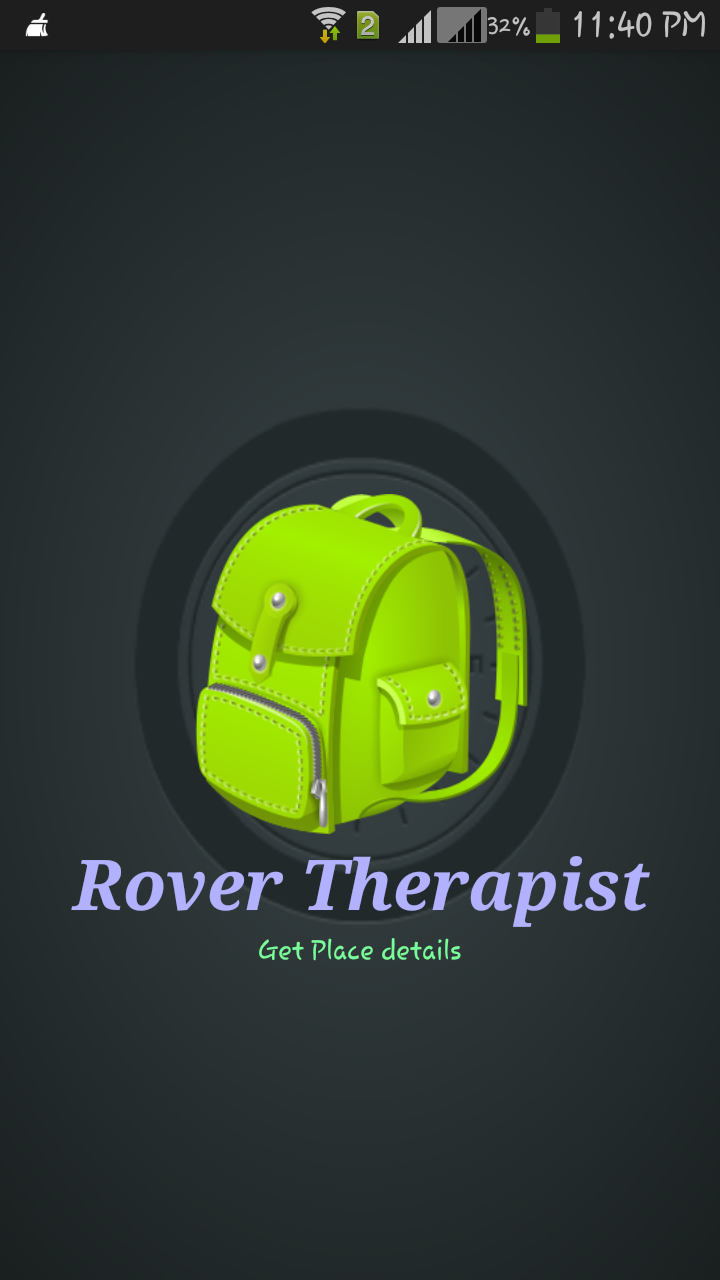
\includegraphics[width=12 cm]{splash}
\caption{Splash Screen}
\end{figure}
\\
\subsubsection{Register User Screen}
\begin{figure}[!htb]
\centering
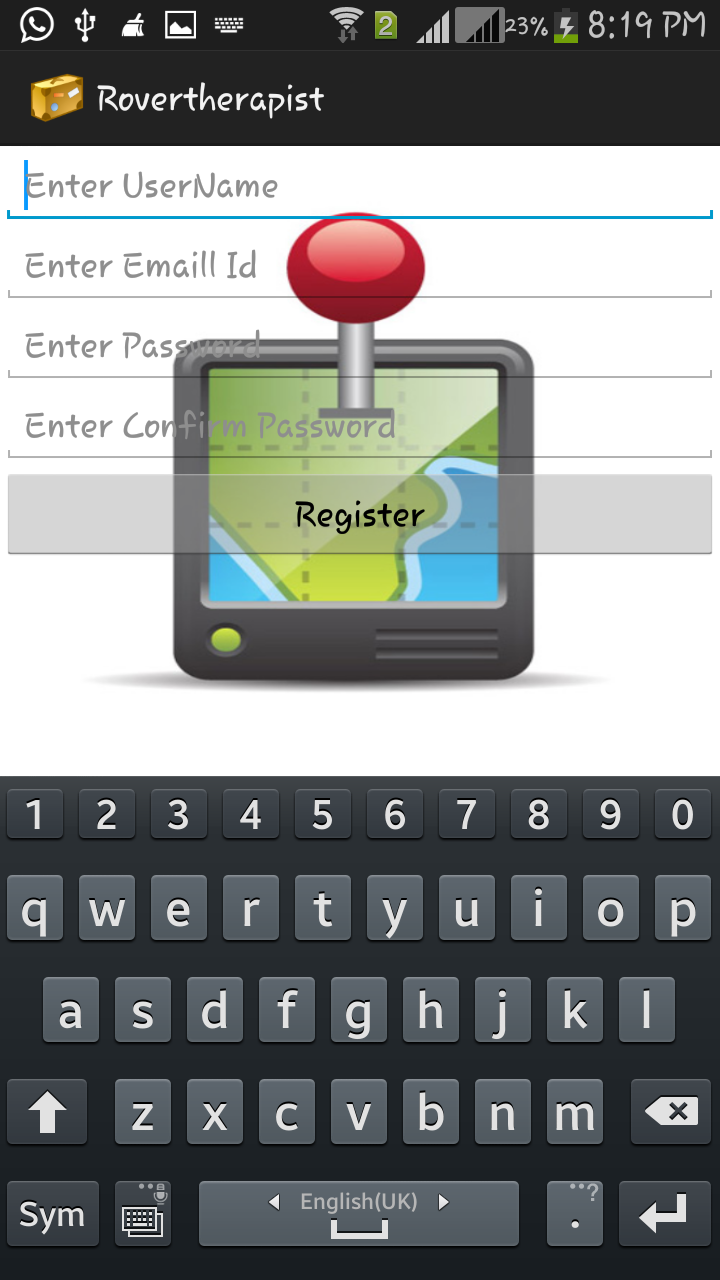
\includegraphics[width=12 cm]{register}
\caption{Register User Screen}
\end{figure}
\\
\subsubsection{Sign in as guest Screen}
\begin{figure}[!htb]
\centering
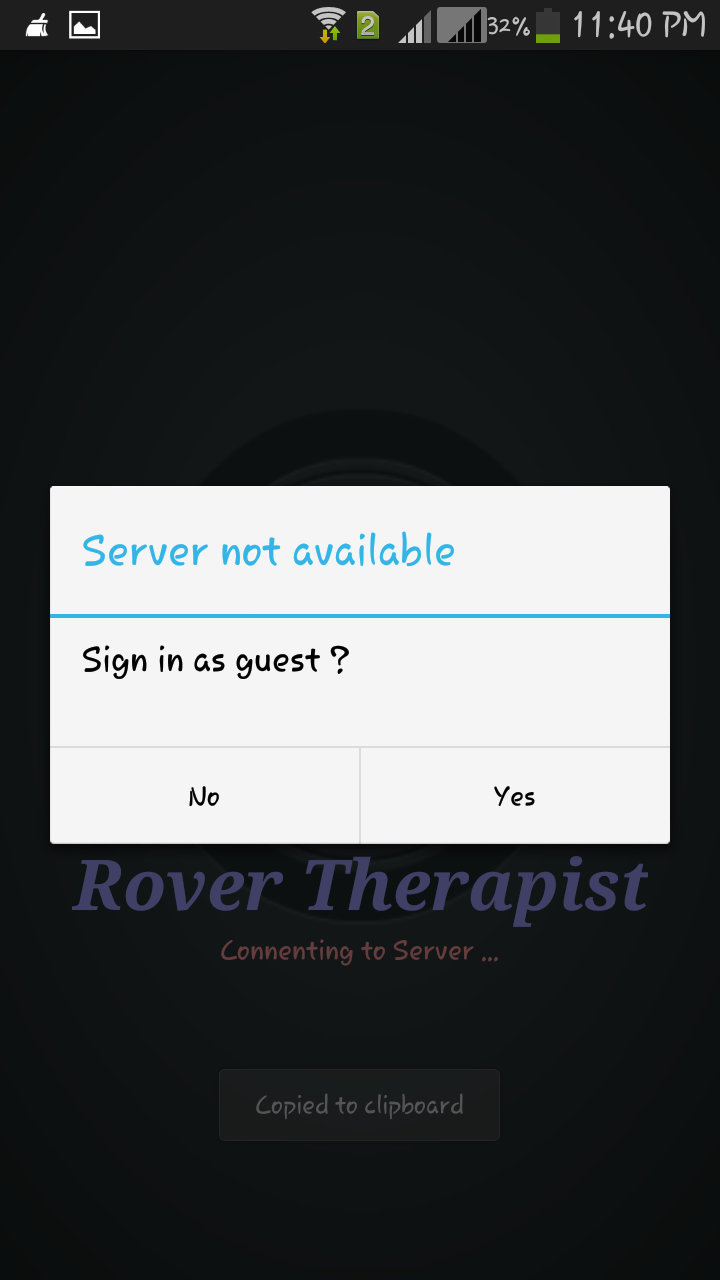
\includegraphics[width=12 cm]{sign}
\caption{Sign In As Guest Screen}
\end{figure}
\\
\subsubsection{Server Connection Parameters Screen}
\begin{figure}[!htb]
\centering
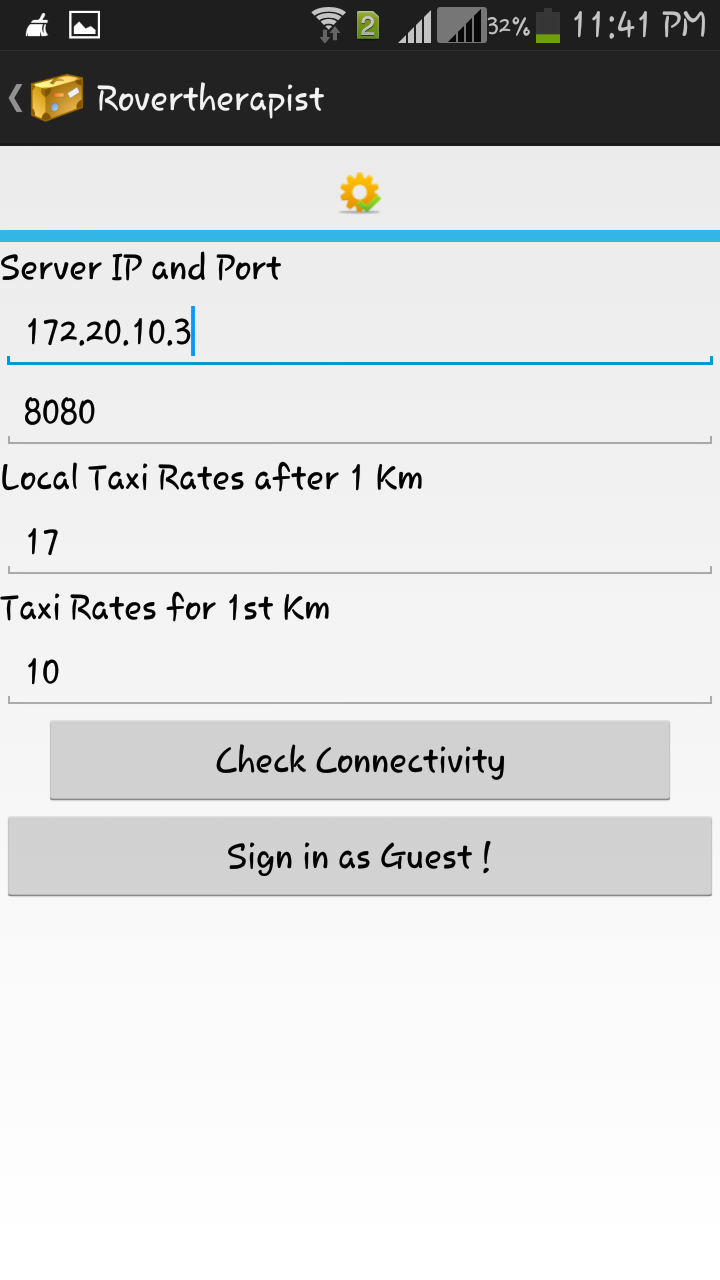
\includegraphics[width=12 cm]{server}
\caption{Server Connection Parameters Screen}
\end{figure}
\\
\subsubsection{List of Attraction Screen}
\begin{figure}[!htb]
\centering
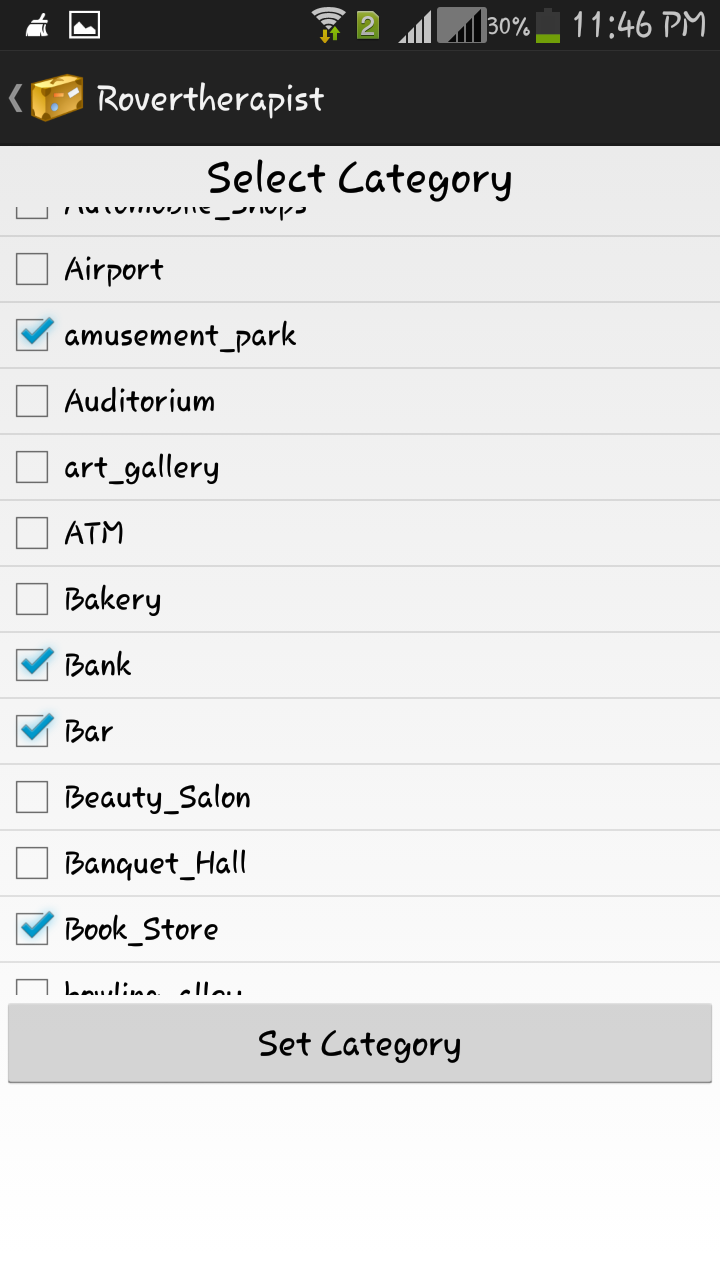
\includegraphics[width=12 cm]{attraction}
\caption{List of Attraction Screen}
\end{figure}
\\
\subsubsection{Direction Screen}
\begin{figure}[!htb]
\centering
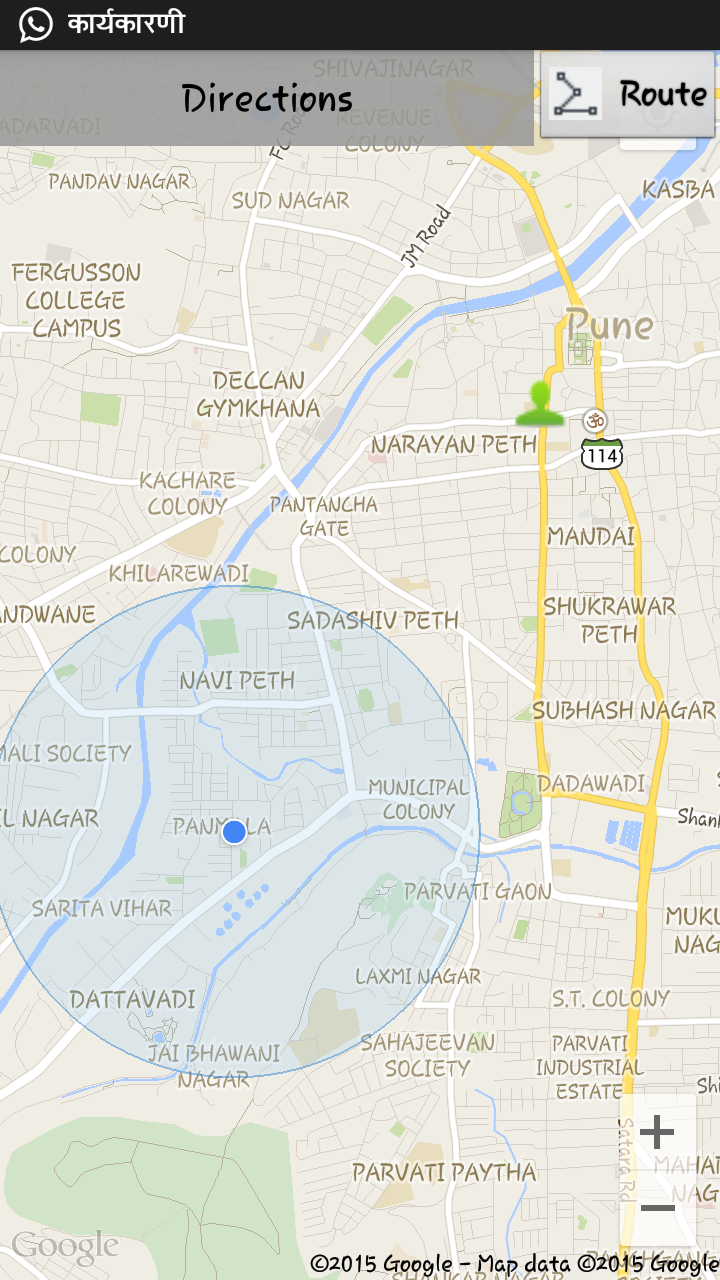
\includegraphics[width=12 cm]{directions}
\caption{Direction Screen}
\end{figure}
\\
\subsubsection{Routes Screen}
\begin{figure}[!htb]
\centering
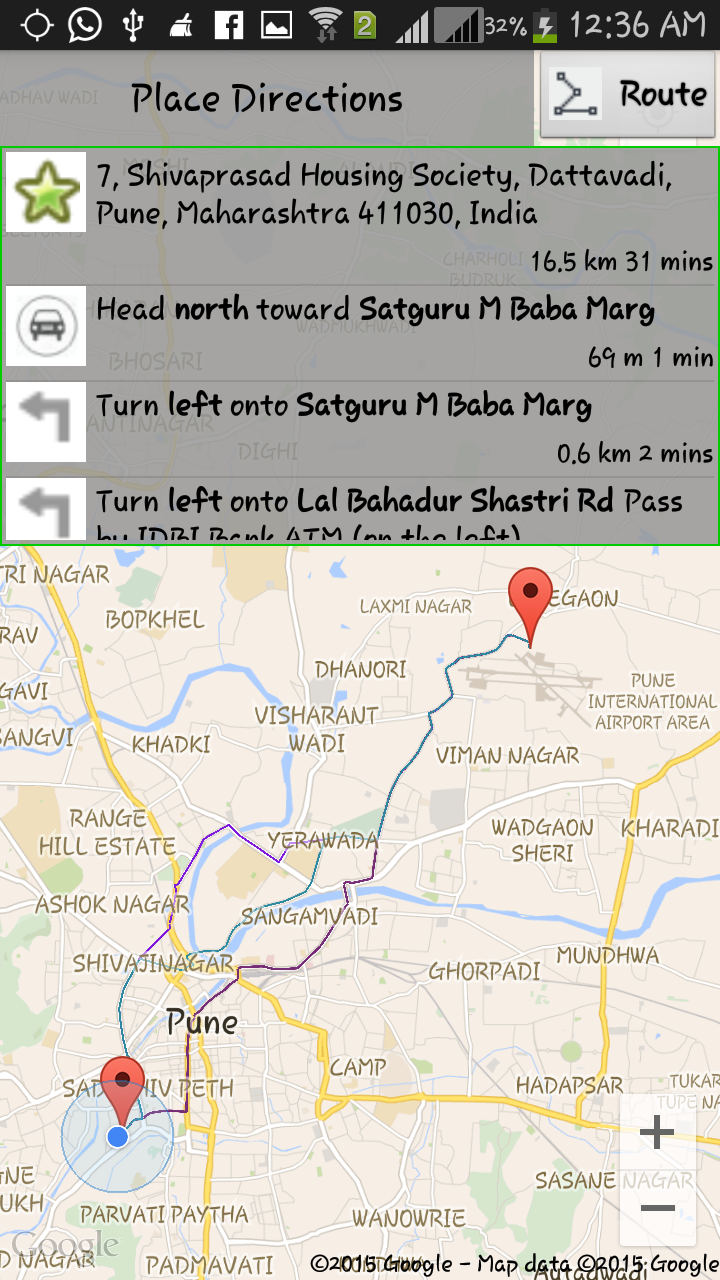
\includegraphics[width=12 cm]{route}
\caption{Route Screen}
\end{figure}
\\
\subsubsection{Weather Screen}
\begin{figure}[!htb]
\centering
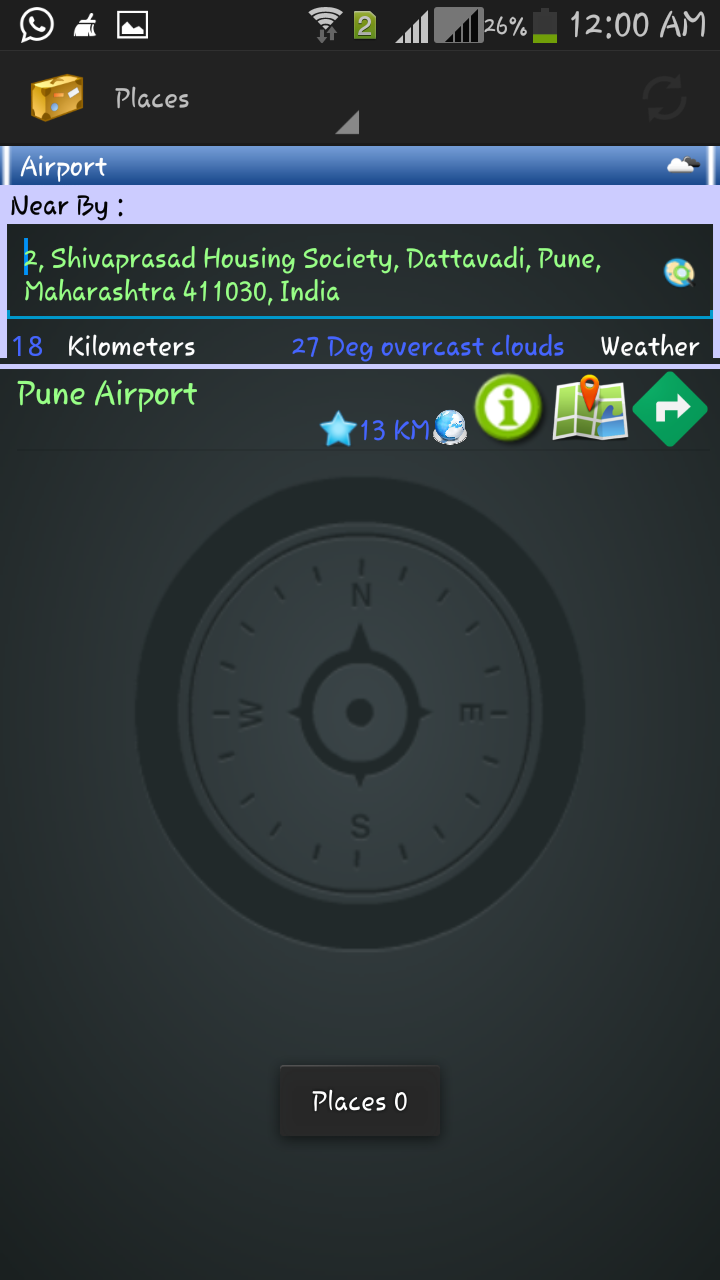
\includegraphics[width=12 cm]{weather}
\caption{Weather Screen}
\end{figure}
\\
\subsubsection{Place Information Screen}
\begin{figure}[!htb]
\centering
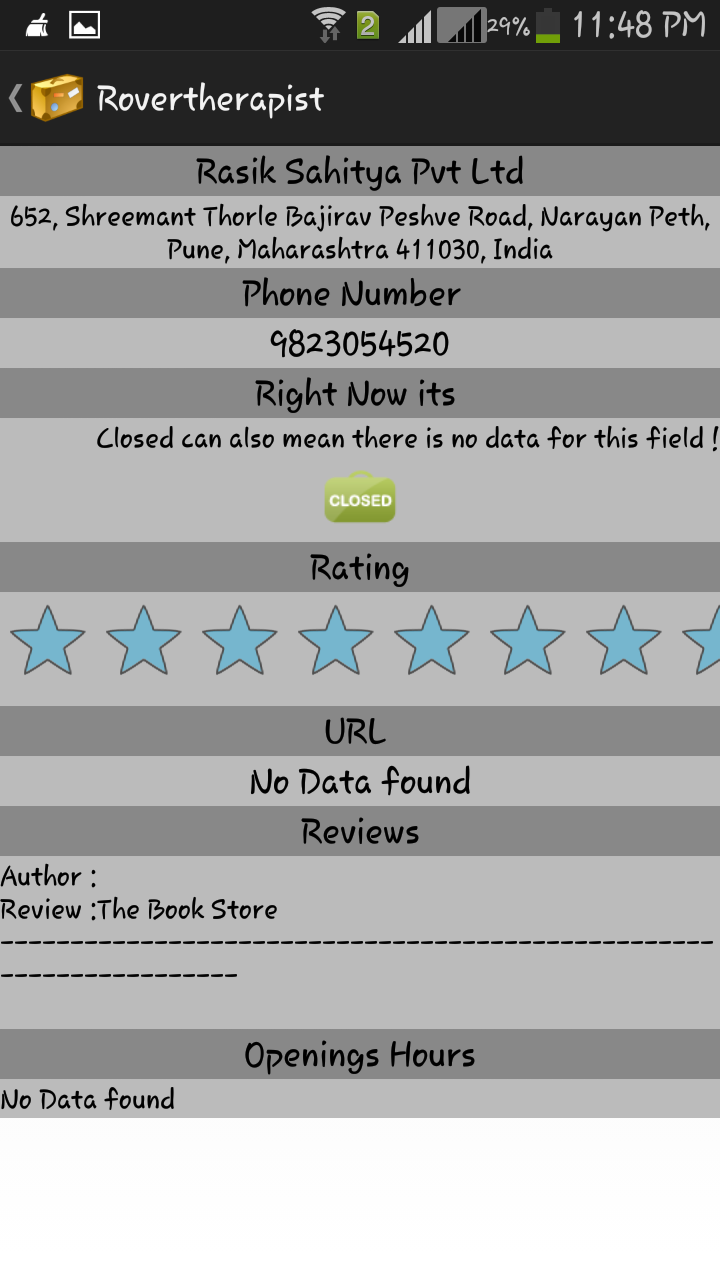
\includegraphics[width=12 cm]{place}
\caption{Place Information Screen}
\end{figure}
\\
\subsubsection{Time Distance and Fare Screens}
\begin{figure}[!htb]
\centering
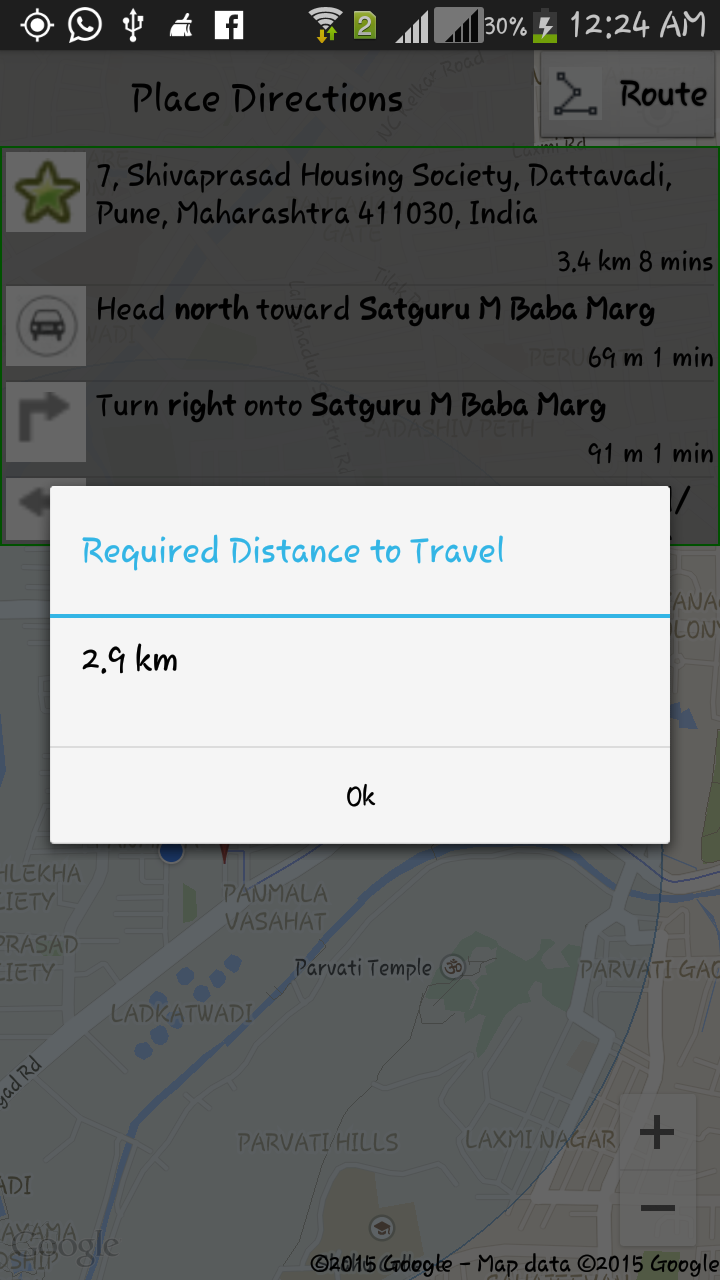
\includegraphics[width=12 cm]{distance}
\caption{Distance to travel Screen}
\\
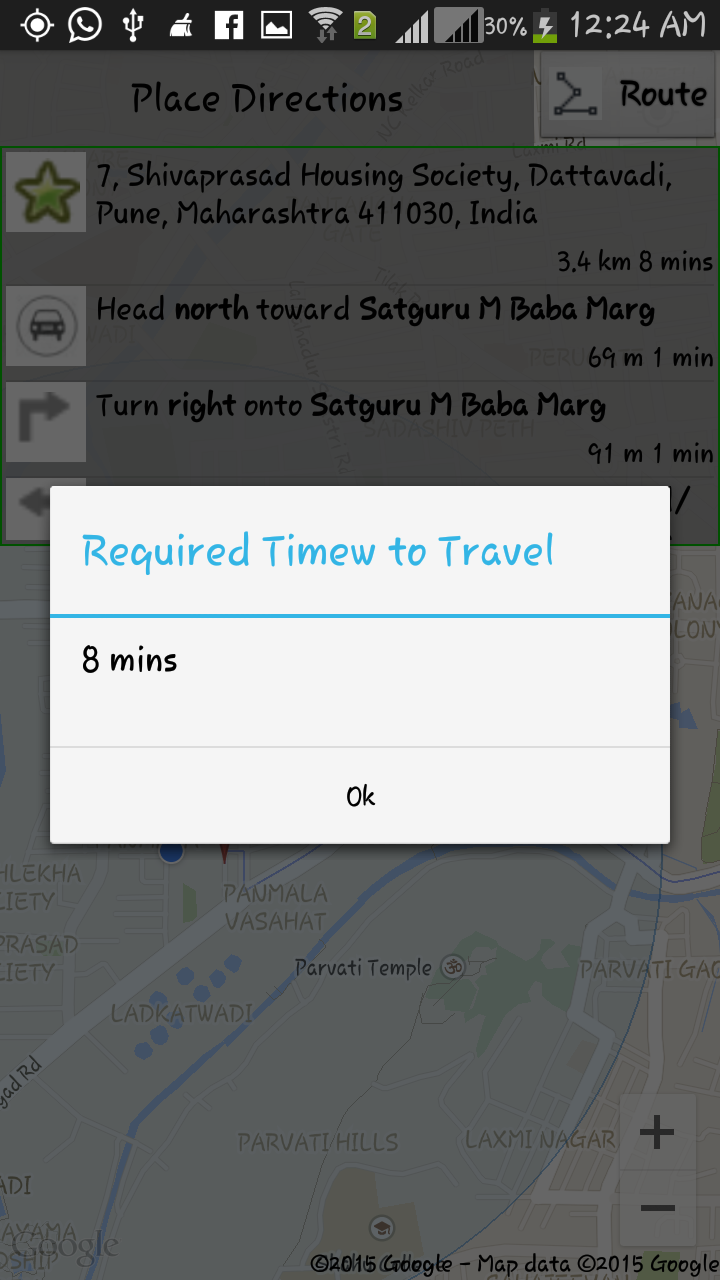
\includegraphics[width=12 cm]{time}
\caption{Time to travel Screen}
\\
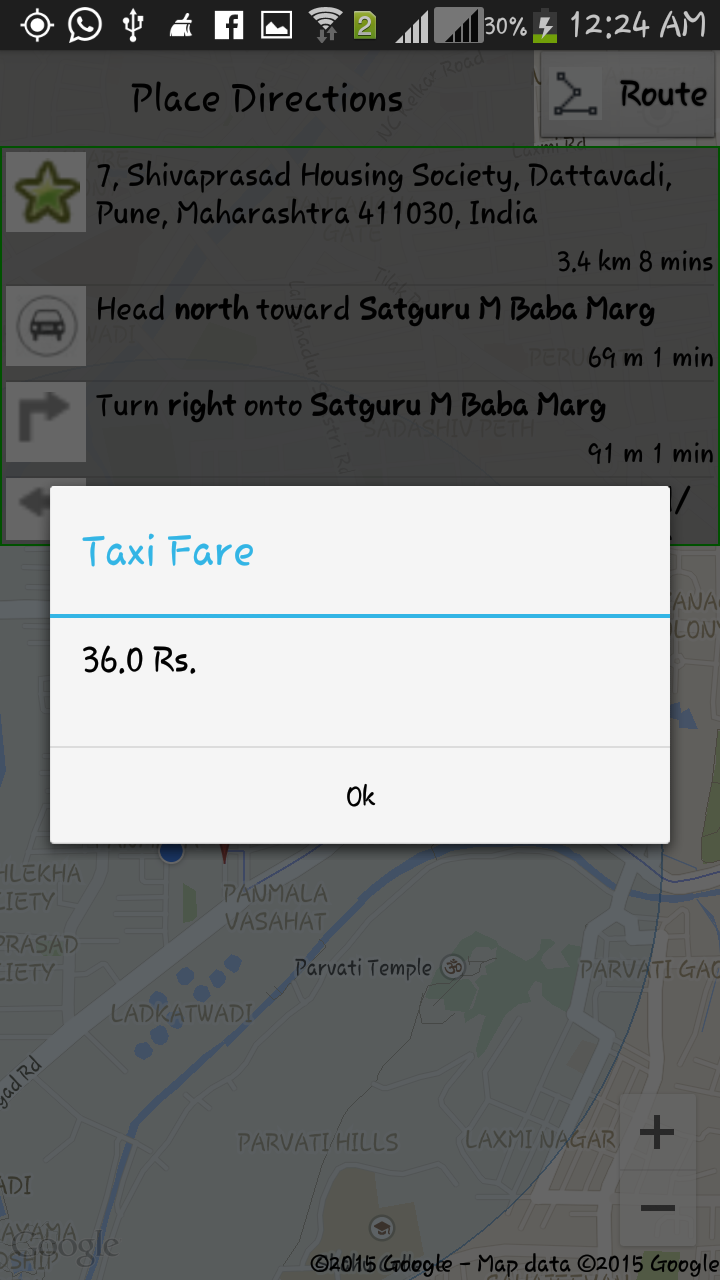
\includegraphics[width=12 cm]{fare}
\caption{Fare Screen}
\end{figure}
\\
\subsubsection{Launch Complaint Screen}
\begin{figure}[!htb]
\centering
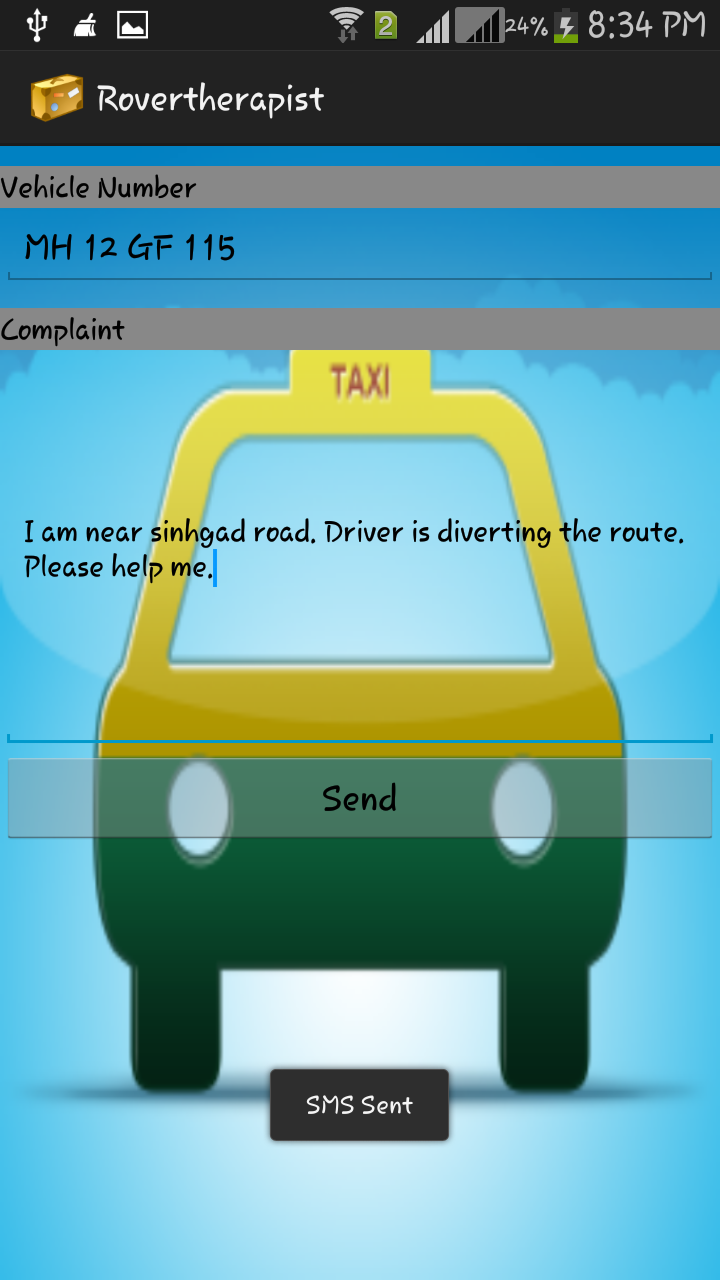
\includegraphics[width=12 cm]{complaint}
\caption{Launch Complaint Screen}
\end{figure}
\\
%---------------------------------------------------------------------------------------------------------

\newpage
\pagestyle{plain}
\begin{center}
\section{TESTING}
\end{center} 
\\
\subsection{MANUAL TEST CASES}
\\
\begin{center}
\vspace{0.1cm}

\newpage
\subsubsection{SPLASH SCREEN}
\begin{center}
\begin{table}
\begin{tabular}{| p{l cm} | p{3 cm} | p{3 cm} | p{3 cm} | p{1 cm} |}
\hline
\textbf{TEST NO.} & \textbf{TEST CASE STEP} & \textbf{EXPECTED OUTPUT} & \textbf{ACTUAL OUTPUT} & \textbf{REMARK} &
\hline
1 & Start the application &	Splash screens should appear & Splash screen appears & Pass &
\hline
\end{tabular}
\caption{Splash Screen Test Cases}
\end{table}
\end{center}

\subsubsection{SIGN IN AS GUEST}
\begin{center}
\begin{table}
\begin{tabular}{| p{l cm} | p{3 cm} | p{3 cm} | p{3 cm} | p{1 cm} |}
\hline
\textbf{TEST NO.} & \textbf{TEST CASE STEP} & \textbf{EXPECTED OUTPUT} & \textbf{ACTUAL OUTPUT} & \textbf{REMARK} &
\hline
1 &	Sign in as guest message->Yes &	Register user screen should appear & Register user screen appears & Pass &
\hline
2 &	Sign in as guest message->No &	Server screen should appear & Server screen appears & Pass &
\hline
\end{tabular}
\caption{Sign In As Guest Screen Test Cases}
\end{table}
\end{center}

\subsubsection{SERVER PARAMETER CONNECTION SCREEN}
\begin{center}
\begin{table}
\begin{tabular}{| p{l cm} | p{3 cm} | p{3 cm} | p{3 cm} | p{1 cm} |}
\hline
\textbf{TEST NO.} & \textbf{TEST CASE STEP} & \textbf{EXPECTED OUTPUT} & \textbf{ACTUAL OUTPUT} & \textbf{REMARK} &
\hline
1 &	Touch the textfields &	Keyboard should appear & Keyboard appears & Pass &
\hline
2 &	Touch the connectivity button & Connection to server should be established & Connection is established & Pass &
\hline
\end{tabular}
\caption{Server Parameter Connection Screen Test Cases}
\end{table}
\end{center}

\subsubsection{MAIN SCREEN}
\begin{center}
\begin{table}
\begin{tabular}{| p{l cm} | p{3 cm} | p{3 cm} | p{3 cm} | p{1 cm} |}
\hline
\textbf{TEST NO.} & \textbf{TEST CASE STEP} & \textbf{EXPECTED OUTPUT} & \textbf{ACTUAL OUTPUT} & \textbf{REMARK} &
\hline
1 &	Touch the menu & Dropdown list should appear & Dropdown list appears & Pass &
\hline
2 &	 & Current location of user should be displayed	 & Current location of user is displayed & Pass &
\hline
3 & Touch the direction symbol & User should be navigated to the direction screen & User is navigated to the direction screen & Pass &
\hline
4 & Touch the information symbol & User should be navigated to the information screen & User is navigated to the information screen	& Pass &
\hline
5 & Touch the location symbol & User should be navigated to the location screen	& User is navigated to the location screen	& Pass &
\hline
\end{tabular}
\caption{Main Screen Test Cases}
\end{table}
\end{center}

\subsubsection{MENU SCREEN}
\begin{center}
\begin{table}
\begin{tabular}{| p{l cm} | p{3 cm} | p{3 cm} | p{3 cm} | p{1 cm} |}
\hline
\textbf{TEST NO.} & \textbf{TEST CASE STEP} & \textbf{EXPECTED OUTPUT} & \textbf{ACTUAL OUTPUT} & \textbf{REMARK} &
\hline
1 &	Touch the change distance option & Distances should appear and as per the distance selected by the user, list of places should appear & Distances appears and as per the distance selected by the user, list of places appears & Pass &
\hline
2 &	Touch the change category option & User should be navigated to the list of attractions screen and as per the attractions selected by the user places on the main screen should appear & User is navigated to the list of attractions screen and as per the attractions selected by the user places on the main screen appears & Pass &
\hline
3 & Touch the launch compliant option & User should be navigated to the complaint screen & User is navigated to complaint screen & Pass &
\hline
4 & Touch the information symbol & User should be able to get a popup of the calculated disatnce and fare & User gets the calculated distance and fare & Pass &
\hline
\end{tabular}
\caption{Menu Test Cases}
\end{table}
\end{center}
\newpage
\subsection{AUTOMATED TEST CASES}
\\
\subsubsection{TEST LOG}
\\
\newpage
\subsubsection{TEST REPORT}
\\

%---------------------------------------------------------------------------------------------------------

\newpage
\pagestyle{plain} 
\begin{center}
\section{CONCLUSION AND FUTURE ENHANCEMENT}
\end{center}
\hspace{0.7 cm} In this project, we have added new features like fare calculations, shortest route, places according to the weather to visit, choice of distance to the available application. We have also created our own database so the user can be guided even if his GPS is off.
\\
\hspace{0.7 cm} Our project is limited to the city. But it can be extended to other cities, states. 
\\

%---------------------------------------------------------------------------------------------------------

\newpage
\pagestyle{plain}
\begin{center}
\section{BIBLOGRAPHY}
\end{center}
\\
\begin{enumerate}
\item Nitin Khondre, Ravi Saini, Ronak Jain, Sarang Suryawanshi, Bushra Quazi, Customer   Relationship Management Using Android Phone in Tourism, International Journal of Emerging Technology and Advanced Engineering.
\\
\item Filipe Andre Gomes Batista, Nuno Rodrigues, and Alexandrino Goncalves, inGuide-Interactive Guide, 2009 3rd IEEE International Conference on Digital Ecosystems and Technologies Future Mobile CRM in Automotive and Tourist Area
\\
\item R. Ivanov On-line GPS Track Simplification Algorithm for Mobile Platforms, Information Technology and control, 2010
\\
\item Monika Bazard, Sonia Bhardwaj, Overview on Android- The New Mobile Operating System, International Journal of Science, Technology and Management Volume 2, Issue 1, April, 2011
\\
\item
\\
\item
\\
\item
\\
\item
\\
\item
\\
\item www.develpoer.android.com
\\
\item www.json.org
\\
\item www.wikipedia.org/wiki/Eclipse_(software)
\\
\item http://en.wikipedia.org/wiki/MYSQL
\\
\item http://en.wikipedia.org/wiki/Apache_Tomcat

%---------------------------------------------------------------------------------------------------------

\end{document}